\documentclass[12pt]{article}
\usepackage[margin=1in]{geometry}
\usepackage{amsmath, amsthm, amssymb, amsfonts, breqn, graphicx}


\theoremstyle{definition}
\newtheorem{problem}{Problem}
\renewcommand*{\proofname}{Solution}
\newenvironment{custompbm}[1]
  {\renewcommand\theproblem{#1}\problem}
  {\endproblem}
\renewcommand{\theenumi}{\alph{enumi}}


\newcommand{\E}{\text{E}}
\newcommand{\V}{\text{Var}}
\newcommand{\Co}[2]{\text{Cov}\left({#1}, {#2}\right)}
\newcommand{\pdf}{\text{pdf}}
\newcommand{\pmf}{\text{pmf}}
\newcommand{\me}{\mathrm{e}}
\newcommand*\diff{\mathop{}\!\mathrm{d}}
\newcommand{\vect}[1]{\boldsymbol{#1}}
\newcommand{\mx}[1][t]{\mu_X({#1})}
\newcommand{\gx}[2]{\gamma_X({#1}, {#2})}


\title{Homework Assignment 10}
\author{Matthew Tiger}


\begin{document}


\maketitle


\begin{problem}
  Plot the energy bills versus time. What kind of trend appears to exist? What type of seasonal
  variation appears to exist? Is a transformation needed to obtain a series that displays constant
  variation?
\end{problem}

\begin{proof}
  See below for a plot of the bills time series data:
  \vskip 0mm
  \center
  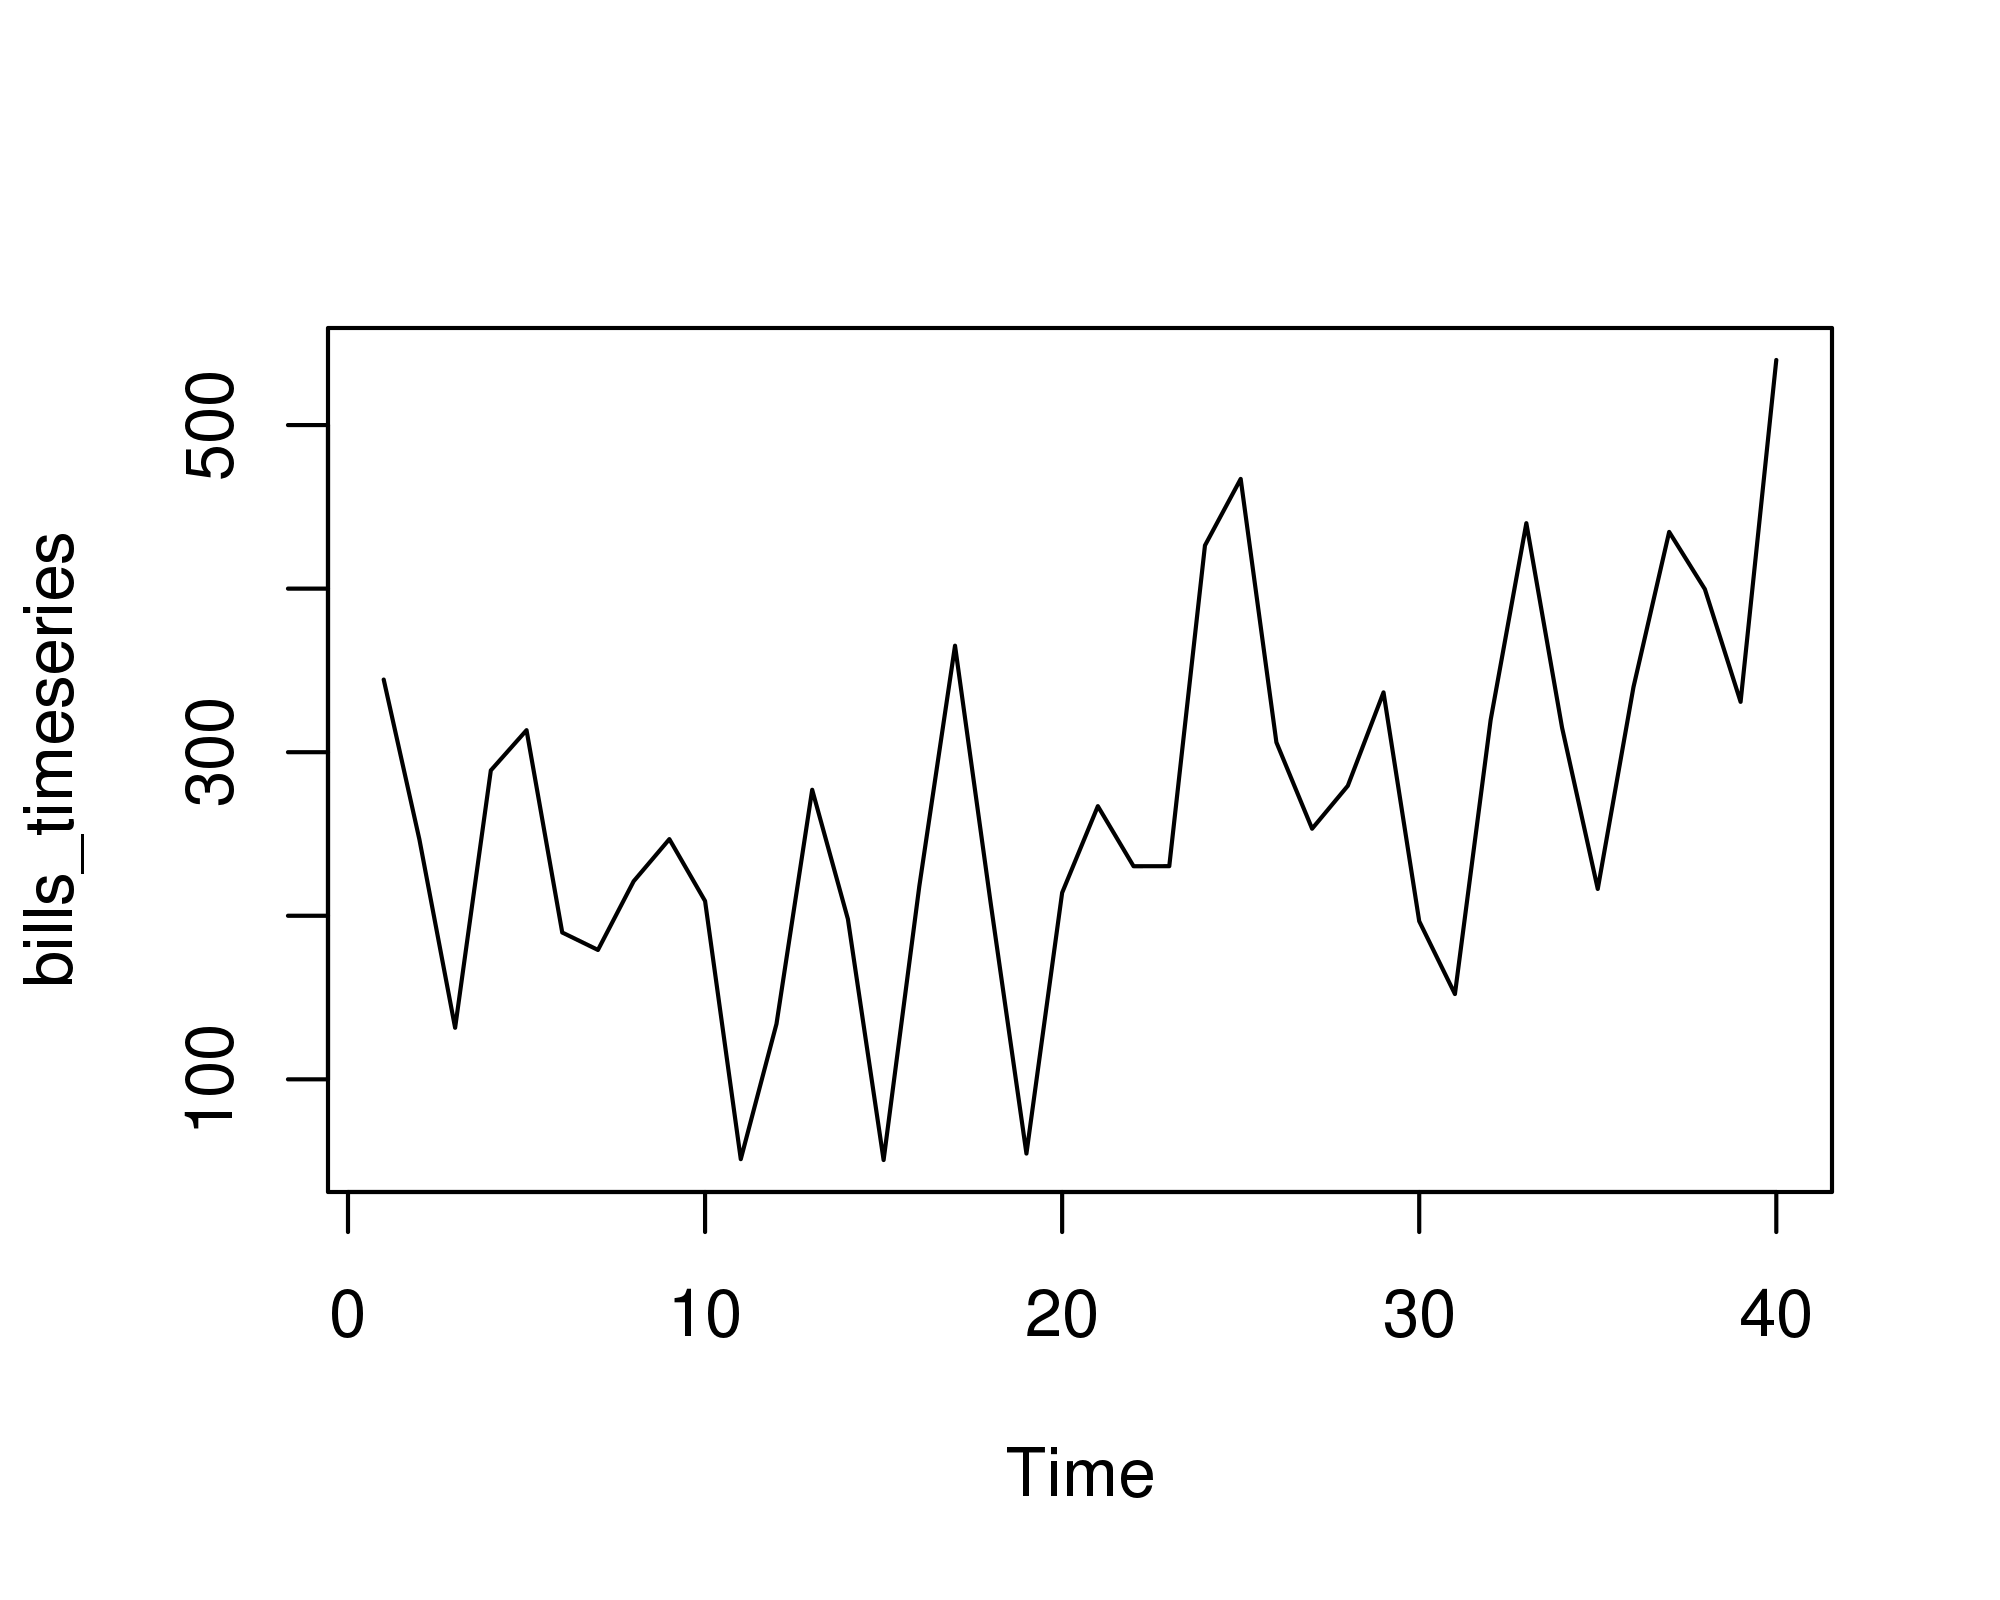
\includegraphics{timeseries}
  \vskip 10mm

  It is clear from the plot that there is both a trend and seasonal variation present
  in the data so a transformation is needed to obtain residuals the represent a
  stationary time series.
\end{proof}


\end{document}
